\chapter{A simple dynamic wake model}
\label{chap:dynwake}
\chaptermark{A simple dynamic wake model}

Wind turbines extract momentum and energy from the wind, generating a wake that travels downstream. These wakes reduce the energy extraction and power production of downstream turbines; however, they also expand through turbulent mixing, thus partially recovering the energy available for subsequent turbines. To provide secondary frequency regulation, wind turbines can be used to modulate energy extraction, changing the properties of the wake generated at the turbine. For instance, if the energy extraction at one turbine is momentarily reduced, increased kinetic energy becomes available in its wake. However, this additional energy only becomes available to the downstream turbine after the flow travel time between these turbines has elapsed. In order to capture such effects quantitatively, we develop a dynamic wake model, drawing on the classic steady-state Jensen wake model~\cite{Katic1986a}, to include the time-varying impact of changing turbine kinetic energy extraction on total wind farm power production.

\section{The dynamics of a wind turbine wake}
\label{sec:dynwake-wakemodel}
We begin by considering the wake behind a single wind turbine. The coordinate system is defined such that the mean inflow velocity $U_\infty$ is directed in the positive $x$ direction, $y$ and $z$ denote the transverse directions, and the origin of the coordinate system is at the center of the rotor swept area. Considering the behavior of the wake in a Reynolds-averaged sense, i.e. solving for the ensemble mean velocity from the unsteady RANS equations, the wake behind a the turbine is governed by the Reynold-averaged mean momentum equation
\begin{equation}
\rho \frac{\partial u_i}{\partial t} + \rho u_j \frac{\partial u_i}{\partial x_j} = - \frac{\partial p}{\partial x_i} - \frac{\partial \tau_{ij}}{\partial x_j} + f_i,
\end{equation}
where $\rho$ is the density of air, $u_i(\mathbf{x},t)$ is the Reynolds-averaged velocity (for convenience we omit the ensemble averaging symbols), $p(\mathbf{x},t)$ is the mean pressure, $f_i(\mathbf{x},t)$ is the turbine thrust force per unit mass, and $\tau_{ij}$ the Reynolds stress tensor.  After neglecting the viscous terms, linearizing the advective term with the average inflow velocity $U_\infty$, i.e. $u_j \frac{\partial }{\partial x_j} = U_\infty \frac{\partial}{\partial x}$, and rewriting in terms of the local velocity deficit $U_\infty\delta_{i1} - u_i({\bf x},t)$, the Reynolds averaged mean momentum equation becomes
%
\begin{equation}
\label{eq:linearized_momentum_deficit}
 \rho \frac{\partial}{\partial t} (U_\infty\delta_{i1} - u_i) +  \rho U_\infty \frac{\partial }{\partial x}  (U_\infty\delta_{i1} - u_i) = \frac{\partial p}{\partial x_i} - f_i + \frac{\partial \tau_{ij}}{\partial x_j},
\end{equation}
As the wake travels downstream, the area of the wake will increase through turbulent mixing. If the expansion rate is determined only by the turbulence properties of the incoming flow, then the effective area of the wake $A(x)$ can be assumed to be a function of only the streamwise distance $x$ from the turbine. As a result, this wake area is constant in time and we implicitly neglect possible dependencies of wake expansion on temporal variations in the thrust coefficient.  Assuming that this effective area --- which will be specified shortly --- is known, the mean velocity deficit $\delta u_i(x,t)$ is defined as
\begin{equation}
\label{eq:area_velocity}
\delta u_i(x,t) = \frac{1}{A(x)}\int_{-\infty}^{\infty} \int_{-\infty}^{\infty}( U_\infty\delta_{i1} - u_i(x,y,z,t)) \, dy \, dz.
\end{equation}
Integrating~\eqref{eq:linearized_momentum_deficit} in the transverse directions, $y$ and $z$, yields
\begin{equation}
\label{eq:averaged_momentum}
\frac{\partial}{\partial t} \left[ \rho A(x) \delta u_i(x,t) \right] + U_\infty \frac{\partial }{\partial x} \left[ \rho  A(x) \delta u_i(x,t)\right] = \frac{\partial \bar{p}}{\partial x}\delta _{i1} - \bar{f}_i ,
\end{equation}
where $\bar{p}(x,t)$ and $\bar{f}_i(x,t)$ denote the transversely averaged pressure and thrust force and $\delta(x)$ is the Dirac delta function. Although the divergence of the Reynolds stress does not enter, the effects of turbulence are encoded in the modeled behavior of $A(x)$. 

Since the thrust force is confined to the rotor disk and the pressure gradient vanishes away from the turbine~\cite{Glauert1935a}, the right hand size of~\eqref{eq:averaged_momentum} only has to be considered in the region near the turbine rotor. The net effect of the pressure gradient and thrust force is therefore modeled as a source of momentum deficit
\begin{equation}
\frac{\partial \bar{p}}{\partial x}\,\delta _{i1} - \bar{f}_i = \rho A(x) \,S_i(t) \, \delta(x),
\end{equation}
where $S_i(t)$ may be time dependent in cases of varying turbine thrust. Substituting  into~\eqref{eq:averaged_momentum}, expanding the spatial derivatives, and dividing by $\rho A(x)$ yields
\begin{equation}
\label{eq:preliminary_deficit}
\frac{\partial \delta u_i}{\partial t} + U_\infty \frac{\partial \delta u_i }{\partial x} = - w(x) \,\delta u_i(x,t) + \,S_i(t) \, \delta(x),
\end{equation}
where the wake expansion rate is
\begin{equation}
w(x) = U_\infty  \frac{1}{A(x)} \frac{d A}{d x}.
\end{equation}

The source strength $S_i(t)$ is specified in a manner consistent with inviscid models of the initial velocity deficit behind the turbine.  In other words, the source strength is determined in such a way that the initial velocity deficit (just after a fluid parcel has passed through the turbine) is $\delta u_i(x=\epsilon) = \delta u_{0i} $, where $\delta u_{0i}$ is the initial velocity deficit known separately as predicted from an inviscid model and $\epsilon$ is a small displacement. To impose this initial velocity deficit, we integrate~\eqref{eq:preliminary_deficit} in $x$ between $x=-\epsilon$, where $\delta u_i(- \epsilon)=0$, and $x=\epsilon$. In this region, the rate of change of $A$ is negligible compared to the effects of the Dirac delta forcing. Hence,~\eqref{eq:preliminary_deficit} becomes $U_\infty  \frac{\partial \delta u_i}{\partial x} = S_i  \delta(x)$, and after integrating we obtain  $\delta u_i(\epsilon)=S_i / U_{\infty}$. Therefore, the source term is specified as $S_i = U_\infty \delta u_{0i}$.

In the unyawed case, the appropriate inviscid model is the actuator disk theory, discussed in Section~\ref{subsec:methods-les-turbine}, which gives an initial velocity deficit $\delta u_{i0} = 2 U_\infty a = 2 U_\infty C_T'/(4+C_T')$ that depends on the induction factor $a$ or the local thrust coefficient $C_T'$. As a result, the only velocity component that remains is in the streamwise direction, and the source term is $S_i(t) = 2 U_\infty a(t) \delta_{i1} = 2 U_\infty C_T'/(4+C_T') \delta_{i1}$. This procedure will properly specify the source of velocity deficit in the unyawed case, but in yawed or tilted cases a different inviscid model is needed, as will be discussed in Chapter~\ref{chap:yaw}.

Since we assume that the wake area is invariant in time, we can consider a steady flow to derive the correct expression for the wake area function
\begin{equation}
A(x)= \frac{\pi D^2}{4} d_w^2(x),
\end{equation}
which is written in terms of $d_w(x)$, the effective diameter of the wake normalized by turbine diameter $D=2R$. After linearizing the advective term, assuming the pressure gradient vanishes in the region sufficiently downstream from the turbine, neglecting the streamwise Reynolds stress, and using the eddy viscosity model, the Reynolds-averaged mean momentum equation for the streamwise velocity $u$ in the region away form the turbine forcing becomes
\begin{equation}
\label{eq:RANS_eddy_viscosity}
U_\infty \frac{\partial u}{\partial x} = \frac{1}{r} \frac{\partial}{\partial r} \left( r \nu_T  \frac{\partial u}{\partial r} \right),
\end{equation}
where $r$ is the distance from the center of the wake and $\nu_T$ is the eddy viscosity. Past research has noted that the far wake of a turbine has a self-similar profile~\cite{Bastankhah2014a}; therefore, the velocity may be written as
\begin{equation}
\label{eq:deficit_profile}
u(x,r) = U_\infty - \delta u(x) W\left(\frac{r}{\ell(x)}\right),
\end{equation}
where $W(\xi)$ is a self-similar function of $\xi = \frac{r}{\ell(x)}$ and $\ell(x) \sim D d_w(x)$ is proportional to the diameter of the wake. 

For a free wake, the eddy viscosity scales with the wake width and the velocity deficit $\nu_T \sim \delta u \, \ell$~\cite{Tennekes1972a}. In the atmospheric boundary layer, however, the appropriate velocity scale is the friction velocity $u_*$, giving the following eddy viscosity
\begin{equation}
\label{eq:eddy_viscosity}
\nu_T(x) = u_* \ell(x).
\end{equation}
Replacing~\eqref{eq:deficit_profile} and~\eqref{eq:eddy_viscosity} into~\eqref{eq:RANS_eddy_viscosity} and expanding the derivatives we obtain
\begin{equation}
-U_\infty \frac{d \delta u}{dx} W + U_\infty \delta u(x)\frac{r }{\ell(x)^2} \frac{d \ell}{dx}W' = -\frac{u_* \delta u(x)}{r} W' -\frac{u_* \delta u(x)}{\ell(x)} W'',
\end{equation}
where primes denote derivatives with respect to $\xi$. Rearranging in dimensionless form
\begin{equation}
\frac{U_\infty}{u_*}  \frac{\ell(x)}{\delta u(x)}  \frac{d \delta u}{dx} W = \left(\frac{U_\infty}{u_*} \frac{d \ell}{dx} \xi  + \frac{1}{\xi}\right)W' +W'',
\end{equation}
we find that in order for the profile to be self-similar, two values must be constant in the wake
\begin{align}
\label{eq:self-similar1}
\frac{U_\infty}{u_*} \frac{d \ell}{dx} &= \text{constant} \\
\label{eq:self-similar2}
\frac{U_\infty}{u_*}  \frac{\ell(x)}{\delta u(x)}  \frac{d \delta u}{dx} &= \text{constant}.
\end{align}

From~\eqref{eq:self-similar1}, we note that $\ell(x) \sim x$ expands linearly with downstream distance, as in the Jensen model~\cite{Jensen1983a, Katic1986a}. We use the linear growth form of the Jensen model, where the dimensionless diameter of the wake $d_w(x) = 1 + 2k_wx/D$ grows at rate determined by an empirical wake expansion coefficient  $k_w$, with two modifications. First, the linear expansion is assumed to begin at $x = 2\Delta_w$ to prevent the wake expansion from occurring within the induction zone imposed by the Gaussian forcing. Second, the equation for the standard Jensen dimensionless wake diameter is ill-posed upstream of the turbine, where it can vanish or become negative. Therefore, we instead use the following modified function that smoothly approximates the linear expansion in the far wake while avoiding becoming less than unity close to the turbine
\begin{equation}
d_w(x) = 1 + k_w\ln \left(1 + \exp \left[\frac{x-2\Delta_w}{R}\right]\right).
\end{equation}
Note that here we follow the approach used in most applications of the Jensen model by assuming that the wake's initial diameter is D rather than the further expanded streamtube diameter $D \sqrt{(1-a)/(1-2a)}$.

While the solution to~\eqref{eq:self-similar2} only requires $\delta u \sim x^n$, we can find the scaling using momentum flux conservation in the far field limit
\begin{equation}
\begin{split}
\int_0^\infty U_\infty \left[ U_\infty - u(x,r) \right] 2 \pi r \, dr &= \int_0^\infty U_\infty \delta u(x) W\left( \xi \right) 2 \pi \ell^2(x) d\xi \\
&= U_\infty \delta u(x) \ell^2(x) C,
\end{split}
\end{equation}
where $C$ is a constant that depends on the initial velocity deficit in the wake $\delta u_0$ and the integral $\int_0^\infty W(\xi) \, d\xi$. Therefore the velocity deficit scales inversely with the square of the downstream distance $\delta u \sim x^{-2}$. Solving the steady-state version of the PDE~\eqref{eq:preliminary_deficit} also provides this scaling.

Furthermore, to model the velocity deficit field in a smooth manner, the Dirac delta function in~\eqref{eq:preliminary_deficit} is replaced by a normalized Gaussian function with characteristic width $\Delta_w=R$.
\begin{equation}
\label{eq:gaussian}
G(x) = \frac{1}{\Delta_w\sqrt{2\pi}} \exp \left({-\frac{x^2}{2 \Delta_w^2}} \right).
\end{equation}
This approach provides a smooth increase of the velocity deficits from zero upstream of the rotor to the desired `wake initial condition' downstream of the rotor region. It also mimics the effect of the pressure gradient inside the streamtube upstream and downstream of the actuator disk. The resulting PDE model equation for the velocity deficit becomes 
\begin{equation}
\label{eq:velocity_deficit}
\frac{\partial \delta u_i}{\partial t} + U_\infty \frac{\partial \delta u_i }{\partial x} = - w(x) \,\delta u_i(x,t) + \,S_i(t) \, G(x).
\end{equation}
Written in this way, the left hand side of~\eqref{eq:velocity_deficit} represents advection of the velocity deficit. The first term on the right hand side, $w(x)\delta u_i(x,t)$, represents transverse diffusion through turbulent mixing, which is characterized by the expansion of the wake area. The forcing term $S_i(t) \, G(x)$ represents turbine thrust and the resulting streamwise pressure distribution around the turbine. Furthermore, to fully specify this model, initial and boundary conditions are needed for the velocity deficit. Since the turbine produces no velocity deficit upstream of the turbine, the inlet boundary condition is $\delta u_i(0, t) = 0$. The initial condition is denoted as $\delta u_i(x,0)$. 

\section{Dynamic unyawed wind farm model}
\label{sec:dynwake-1d}
In the present discussion, we will consider regular rectangular wind farms of $N$ rows and $M$ columns in aligned and staggered configurations, as shown in Figure~\ref{fig:wake_model}(a)--(b). In both cases, we will also only consider unyawed configurations, where the turbine is directly aligned with the incoming wind. Each column $m \in 1, \hdots, M$ of turbines is defined as a set of turbines aligned with the prevailing wind direction. Ordering turbines in each column from inlet to outlet, each row $n \in 1, \hdots, N$ of turbines is defined as the set of $n$-th turbines in all columns. Although this paper only considers regular arrangements, the proposed model can be supplemented to include irregular farms using the more general superposition approach of the classic Jensen model~\cite{Katic1986a}. To further simplify the approach in the current work and allow for better averaging in LES evaluations (cf. Section~\ref{subsec:dynwake-1d-validation}), we consider each row of turbines collectively, as shown in Figure~\ref{fig:wake_model}(b), which effectively neglects the spanwise merging of wakes. This results in a one-dimensional model where the streamwise coordinate $x$ is aligned with the prevailing wind and the streamwise extent of the farm is limited to $x \in [0, L]$, where $x=0$ is several rotor diameters upstream of the first turbine and $x=L$ is several rotor diameters downstream of the last turbine. The wind speed at $x=0$ is denoted as $U_\infty$, and the streamwise location of each row is denoted as $s_n$. In Chapters~\ref{chap:yaw} and~\ref{chap:rhc2} we will relax some of these restrictions to provide a more general theory for yawed turbines in arbitrary arrangements. 

\begin{figure}
\centering
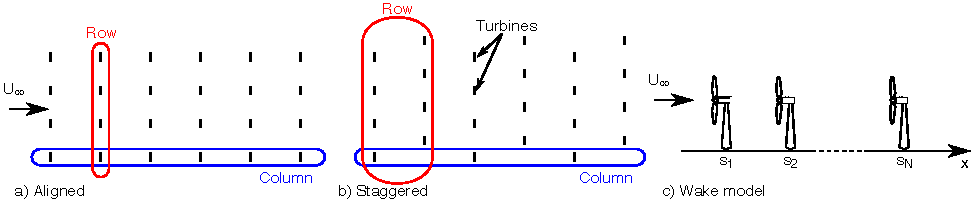
\includegraphics[width=\textwidth]{./fig/wake_model_final.pdf}
\caption{Diagrams of (a) an aligned and (b) a staggered wind farm showing definitions of rows and columns and (c) a wake model showing definitions of the streamwise coordinate x and the turbine locations $\text{s}_\text{n}$. The aligned and staggered wind farms have the same number of turbines, but the staggered arrangement has twice as many columns and double the distance between rows.}
\label{fig:wake_model}
\end{figure}

Since we are only considering the unyawed case, the forcing is only in the steamwise direction and the index notation can be dropped from the discussion of Section~\ref{sec:dynwake-wakemodel}. Instead, the equations are indexed by turbine row $n$ and some equations must be written in terms of the distance from the turbine rotor $x-s_n$. We follow the simplified approach of the Jensen model~\cite{Katic1986a} by first computing the wake deficit velocity $\delta u_n(x,t)$ for each turbine $n$ as if each turbine was on its own, i.e. based on the same freestream velocity $U_\infty$. As in Section~\ref{subsec:dynwake-conclusions}, time-dependency is included by allowing the  thrust coefficient of each turbine  to depend on time  and describing the associated evolution of the wake deficit velocity $\delta u_n(x,t)$ based on the momentum equation. The velocity deficits of all turbines are then superposed using the common ``square-superposition" approach~\cite{Katic1986a}. 

For completeness, we present the one-dimensional wake model for unyawed turbines in a wind farm with all relevant details. The streamwise velcity deficit of the $n$-th turbine is governed by
\begin{equation}
\label{eq:delta_un}
\frac{\partial \delta u_n}{\partial t} + U_\infty \frac{\partial \delta u_n}{\partial x} = -w_n(x) \delta u_n(x,t) + f_n(x,t),
\end{equation}
where $w_n(x)$ is the wake decay function and $f_n(x,t)$ is a forcing function used to account for the effect of the turbine on the flow field. The wake decay function
\begin{equation}
w_n(x) = 2 \frac{U_\infty}{d_n(x)} \frac{d}{dx}d_n(x)
\end{equation}
is determined by the wake diameter normalized by the rotor diameter 
\begin{equation}
d_n(x) = 1 + k_n\ln \left(1 + \exp \left[\frac{x-s_n-2\Delta_w}{R}\right]\right),
\end{equation}
where $k_n$ is the wake expansion coefficient of the $n$-th turbine. The forcing function is specified as
\begin{equation}
\label{eq:forcing}
f_n(x,t) = 2 U_\infty^2  \frac{C_{Tn}'(t)}{4 + C_{Tn}'(t)} G(x-s_n),
\end{equation}
where $G(x)$ is the same Gaussian function in~\eqref{eq:gaussian}.

Equations~\eqref{eq:delta_un}--\eqref{eq:forcing} above describe the time-varying behavior of a wake generated by a single turbine row. The squared deficits~\cite{Katic1986a} are superposed to calculate the streamwise velocity at position $x$ and time $t$
\begin{equation}
\label{eq:u}
u(x,t) = U_\infty - \left(\sum_{m=1}^N \delta u_m^2(x,t)\right)^{1/2}.
\end{equation}
The estimated velocity at the $n$-th turbine row $\hat{u}_n$ is then found using
\begin{equation}
\label{eq:estimated_velocity} 
\hat{u}_n (t) = \int_0^L  u(x,t) G(x - s_n) \, dx.
\end{equation}
Note that we use the same Gaussian shape function as an integration kernel for this superposition in order to maintain smoothness in the adjoint fields discussed in Chapters~\ref{chap:rhc} and~\ref{chap:rhc2}. Finally, the total estimated power $\hat{P}_n$ of the $M$ turbines in row $n$ is
\begin{equation}
\label{eq:estimated_power_row}
\hat{P}_n =  M \frac{1}{2}\rho \frac{\pi D^2}{4} C'_{Pn} \hat{u}_n^3.
\end{equation}
where $C'_{Pn}$ is the local power coefficient. 

Using simple momentum theory (see Section~\ref{subsec:methods-les-turbine}), which assumes idealized conditions, $C_P' = C_T'$.  These idealized conditions assume that the electrical power generated by the turbine is proportional to the power extracted from the flow and the control actions do not significantly affect the aerodynamic efficiency of the blades~\cite[Appendix A]{Goit2015a}. Aerodynamic losses could also be taken into account by reducing the local power coefficient $C_P' \approx \alpha C_T'$ by a constant factor $\alpha$~\cite{Stevens2014b}. For example, a wind turbine operating at a thrust coefficient of $C_T = 0.75$ and $C_P = 0.45$ would use $\alpha = 0.8$. 

This formulation recovers the classical steady-state Jensen model for a single column if one uses a steady local thrust coefficient and appropriate expressions for the shape function and the normalized wake diameter. Specifically, the use of a Dirac delta function instead of the Gaussian $G(x-s_n) \to \delta(x-s_n)$ restores the step change in velocity deficit at the turbine. The wake expansion function $d_n(x) = 1 + 2k_n(x-s_n)/D$ restores the unmodified linear wake growth. Taken together, the above equations yield a nonlinear model with $N$ inputs $C_{Tn}'$, $N$ outputs $\hat{P}_n$, and a set of $N$ PDEs. While this system is infinite-dimensional, seeking solutions to this model using finite-differencing; this leads to 1,750 states for the relatively coarse grid resolution of 28 m and wind farm size $N=7$ used in this study.

\subsection{Validation --- Wind farm startup}
\label{subsec:dynwake-1d-validation}
We now validate the model by comparing the local velocities at each row estimated by the time-varying one-dimensional wake model to velocities obtained from LES of wind farms at startup. These simulations were performed by Pieter~Bauweraerts using KU Leuven's LES code SP-WIND~\cite{Goit2015a, Calaf2010a, Munters2016a}, which shares many numerical details with LESGO.  Unlike LESGO, however, it uses four-stage fourth-order Runge-Kutta time integration, fourth-order energy conserving finite differencing in the vertical direction. SP-Wind uses shifted periodic boundary conditions for the precursor domain~\cite{Munters2016a} to reduce the production of unrealistically long streamwise streaks in the precursor domain. The Smagorinsky subgrid-stress model~\cite{Smagorinsky1963a} with wall damping is used.

For the startup validation, the prescribed surface roughness parameter is $z_{0} = 0.1$ m. Both the wind farm and the precursor domains use the same constant pressure gradient yielding an average of $U_\infty = 9$ m/s at hub height. The precursor domain and wind farm domains have lengths of $13.3$ km in the streamwise direction, 5 km in the spanwise direction, and 1 km in the vertical direction. The number of gridpoints in each domain is $576 \times 256 \times 128$, which corresponds to grid sizes of 23 m $\times$ 20 m $\times$ 8 m in the streamwise, spanwise, and vertical directions, respectively. In the precursor domain, the recycling region is the first 8.7 km and the fringe forcing region is the last 2 km. In the wind farm domain, the first row of turbines is located 1.4 km from the beginning of the domain and the fringe forcing region is the last 2 km. 

 The simulations are started from a fully-developed neutral atmospheric boundary layer, to which the wind farm actuator disk forcing is introduced as a step change in $C_T'$ from 0 to 1.33. Both aligned and staggered arrangements are considered. The aligned wind farm is composed of $N=14$ rows of $M=10$ turbines. Each turbine has a rotor diameter of $D=100$ m and a hub height of 100 m. The spacing between turbines is $7D$ in the streamwise direction and $5D$ in the spanwise direction. The staggered wind farm uses the same configuration with alternating rows offset by half the spanwise spacing in the spanwise direction. This can be viewed as modeling only one streamwise column of turbines and multiplying by the number of columns. Startup is simulated for 20 different initial conditions, which are generated by the same atmospheric boundary layer simulation but separated by approximately one wind farm flow-through time to produce sufficient independence between inflow conditions. Averaging over spanwise columns and 20 simulations results in an average over a total of 200 samples.

\begin{figure}[h]
\centering
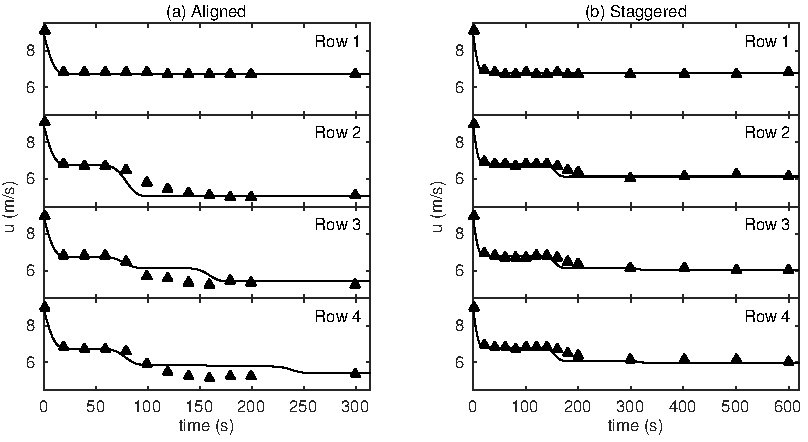
\includegraphics[width=\textwidth]{./fig/startup.pdf}
\caption{Comparison of wake model (---) and LES  averaged over spanwise rows and 20 simulations ($\blacktriangle$) for a wind farm at startup. Local turbine velocities of rows 1--4 are shown as a function of time for (a) aligned and (b) staggered wind farms. The initial decline in velocity in each row is produced by the startup induction of the turbines. Subsequent declines in velocity at downstream rows are produced as the wakes from upstream turbines impact the turbine rotor plane.}
\label{fig:compare}
\end{figure}

The wake model is evaluated numerically using four-stage fourth-order Runge-Kutta time integration with third-order upwind biased spatial discretization, 28 m grid spacing, and a CFL number of 0.99. The parameters $U_\infty$ and $k_n$ must be chosen to describe the flow conditions in the atmospheric boundary layer. In this validation, these parameters are chosen such that the estimated velocities of the steady-state version of the wake mode match the time-averaged velocities from the same wind farm configurations operating at a constant $C_T'=1.33$. The inlet velocity is chosen as $U_\infty = \overline{u}_1(4+C_T')/4$, where $ \overline{u}_1$ is the time-averaged local velocity of the first row of turbines as measured in LES. This results in $U_\infty = 8.93$ m/s for the aligned case and $U_\infty = 9.04$ m/s for the staggered case. The wake expansion coefficients $k_n$ are chosen so that the predicted velocity at downstream rows match the time-averaged LES measurements. The wake model for the staggered case uses only seven rows of turbines with twice the streamwise spacing. 

The time evolution of the velocities at rows 1--4 for a wind farm startup beginning at $t=0$ is shown in Figure~\ref{fig:compare}, where the estimated turbine velocity $\hat{u}_n$ is compared to the streamwise velocity at the center of the turbine rotor averaged over 20 LES. As the model farm and LES start up, the wind speed in all rows initially declines exponentially from the inlet velocity $U_\infty$ to the expected rotor-averaged velocity $4/(4+C_T') U_\infty$. Subsequent declines in velocity at downstream rows are produced as the wakes from upstream turbines impact the turbine rotor plane. Figure~\ref{fig:compare} shows that the wake model captures the wind farm startup response behavior, although there are some obvious differences between the predictions and measurements. For example, assuming a constant advection speed of $U_\infty$ leads to an under-estimate of the advection time between turbines. Maintaining the nonlinear advection speed produces a more accurate wind speed prediction in the wake; however, the concomitant nonlinearity would lead to added complexity and cost in the subsequent control design and implementation. 

\section{Conclusion}
\label{subsec:dynwake-conclusions}
In this chapter, we first developed a simple one-dimensional PDE model of the velocity deficits $\delta u_i(x,t)$ in the wake behind a turbine. This model requires as input the results from inviscid flow past a turbine to specify the forcing term in the PDE. We then apply the model to predict the time evolution of velocity deficits in regularly-arranged wind farms where each turbine is unyawed and compare the model to ensemble and spanwise-averaged large eddy simulations of a wind farm at startup. The performance in Figure~\ref{fig:compare} suggests that the dynamic behavior is adequately captured for a closed-loop control design, where the feedback accommodates small errors. Therefore, this model will be used in the next section for designing controllers for secondary frequency regulation. 
